\section{Data and Methodology}

% \subsection{Which methods are aplied to investigate our problem}
% \begin{itemize}
%     \item RSTF deconvolution from real data for inversion \cite{RSTFVallée2004}.
%     \item Teleseismic phase picking and preparation of the data for inversion.
%     \item Finite-fault kinematic inversion using teleseismic and RSTF data to get slip distribution for both the 2015 and 2025 
%     earthquakes \cite{Vallée2003inversion}.
%     \item Details of these methods will be provided in the supporting information section. 
% \end{itemize}

\subsection{Data}
\begin{itemize}
    \item Continuous three-component waveform time series and their associated metadata for both the 2015 and 2025 events were retrieved from GEOSCOPE and
 other broadband databases, covering networks \textsc{iu}, \textsc{ii}, \textsc{gt}, \textsc{g}, \textsc{ge}, \textsc{dk}, and \textsc{cn} via the \texttt{FetchData}
  utility.
    \item We selected $P$- and $SH$-wave recordings from stations located within an epicentral distance range of $30^\circ$ to $80^\circ$ for both earthquakes.
     The selected array provides well-distributed azimuthal coverage in each case; their spatial distribution is illustrated in 
     Figure~S\ref{fig:2015_tele_station} (for the 2015 event) and Figure~S\ref{fig:2025_tele_station} (for the 2025 event).
    \item A bandpass filter of 0.005 to 0.2 Hz was applied to the obtained data to remove high-frequency noise and low-frequency trends and a combination of
     automated and manual phase picking was performed to identify the arrival times of the $P$ and $SH$ waves. The picked phases were then used to window the 
     data for subsequent analysis. 
    \item For RSTF deconvolution, we retrieved data for a radius of 40 degrees around the epicentres of the 2015 and 2025 earthquakes for same set of networks
    as we used for teleseismic data but at regional to teleseismic distances. We had good azimuthal coverage of the data for both earthquakes. Their spatial 
    distribution is illustrated in Figure~S\ref{fig:2015_rstf_station} (for the 2015 event) and Figure~S\ref{fig:2025_rstf_station} (for the 2025 event).
    \item For RSTF analysis, we selected the same earthquake which happened on 05/04/2025 as our EGF for both 2015 and 2025 events. To qualify as a good EGF, the earthquake should be 
    smaller, have a similar focal mechanism and be located close to the mainshock. This mentioned earthquake is selected as EGF because it satisfies all the
    mentioned criteria.
    \item The retrieved data were preprocessed by removing the instrument response and applying a bandpass filter between 0.0125 and 0.02~Hz. After that
    Love-wave windows were picked. 
    \item Then Relative Source Time Functions (RSTFs) were calculated via the deconvolution method of \cite{RSTFVallée2004} which will be served as input data
     for the finite-fault inversion.
    \item The RSTFs (Fiugure~\ref{fig:2015_rstf} and Figure~\ref{fig:2025_rstf}) show a clear azimuthal dependence, with a stretched profile toward the east 
    and a compressed profile toward
     the west. This pattern is consistent with the directivity effect caused by rupture propagation from west to east
      \cite{Aderhold2016}. The same pattern is observed for both the 2015 and 2025 earthquakes, suggesting that the two events
       had a similar rupture propagation direction.
    \item However, the RSTFs for the 2025 earthquake show stronger stretching and compression compared to those of the 2015 earthquake.
     This suggests that the 2025 rupture was more complex and lasted longer than the 2015 rupture.

    % \begin{figure}[H]
    %     \centering

    %     \resizebox{0.9\textwidth}{!}{
    %         \begin{minipage}{\textwidth}
    %             \begin{subfigure}{0.5\textwidth}
    %                 % \centering
    %                 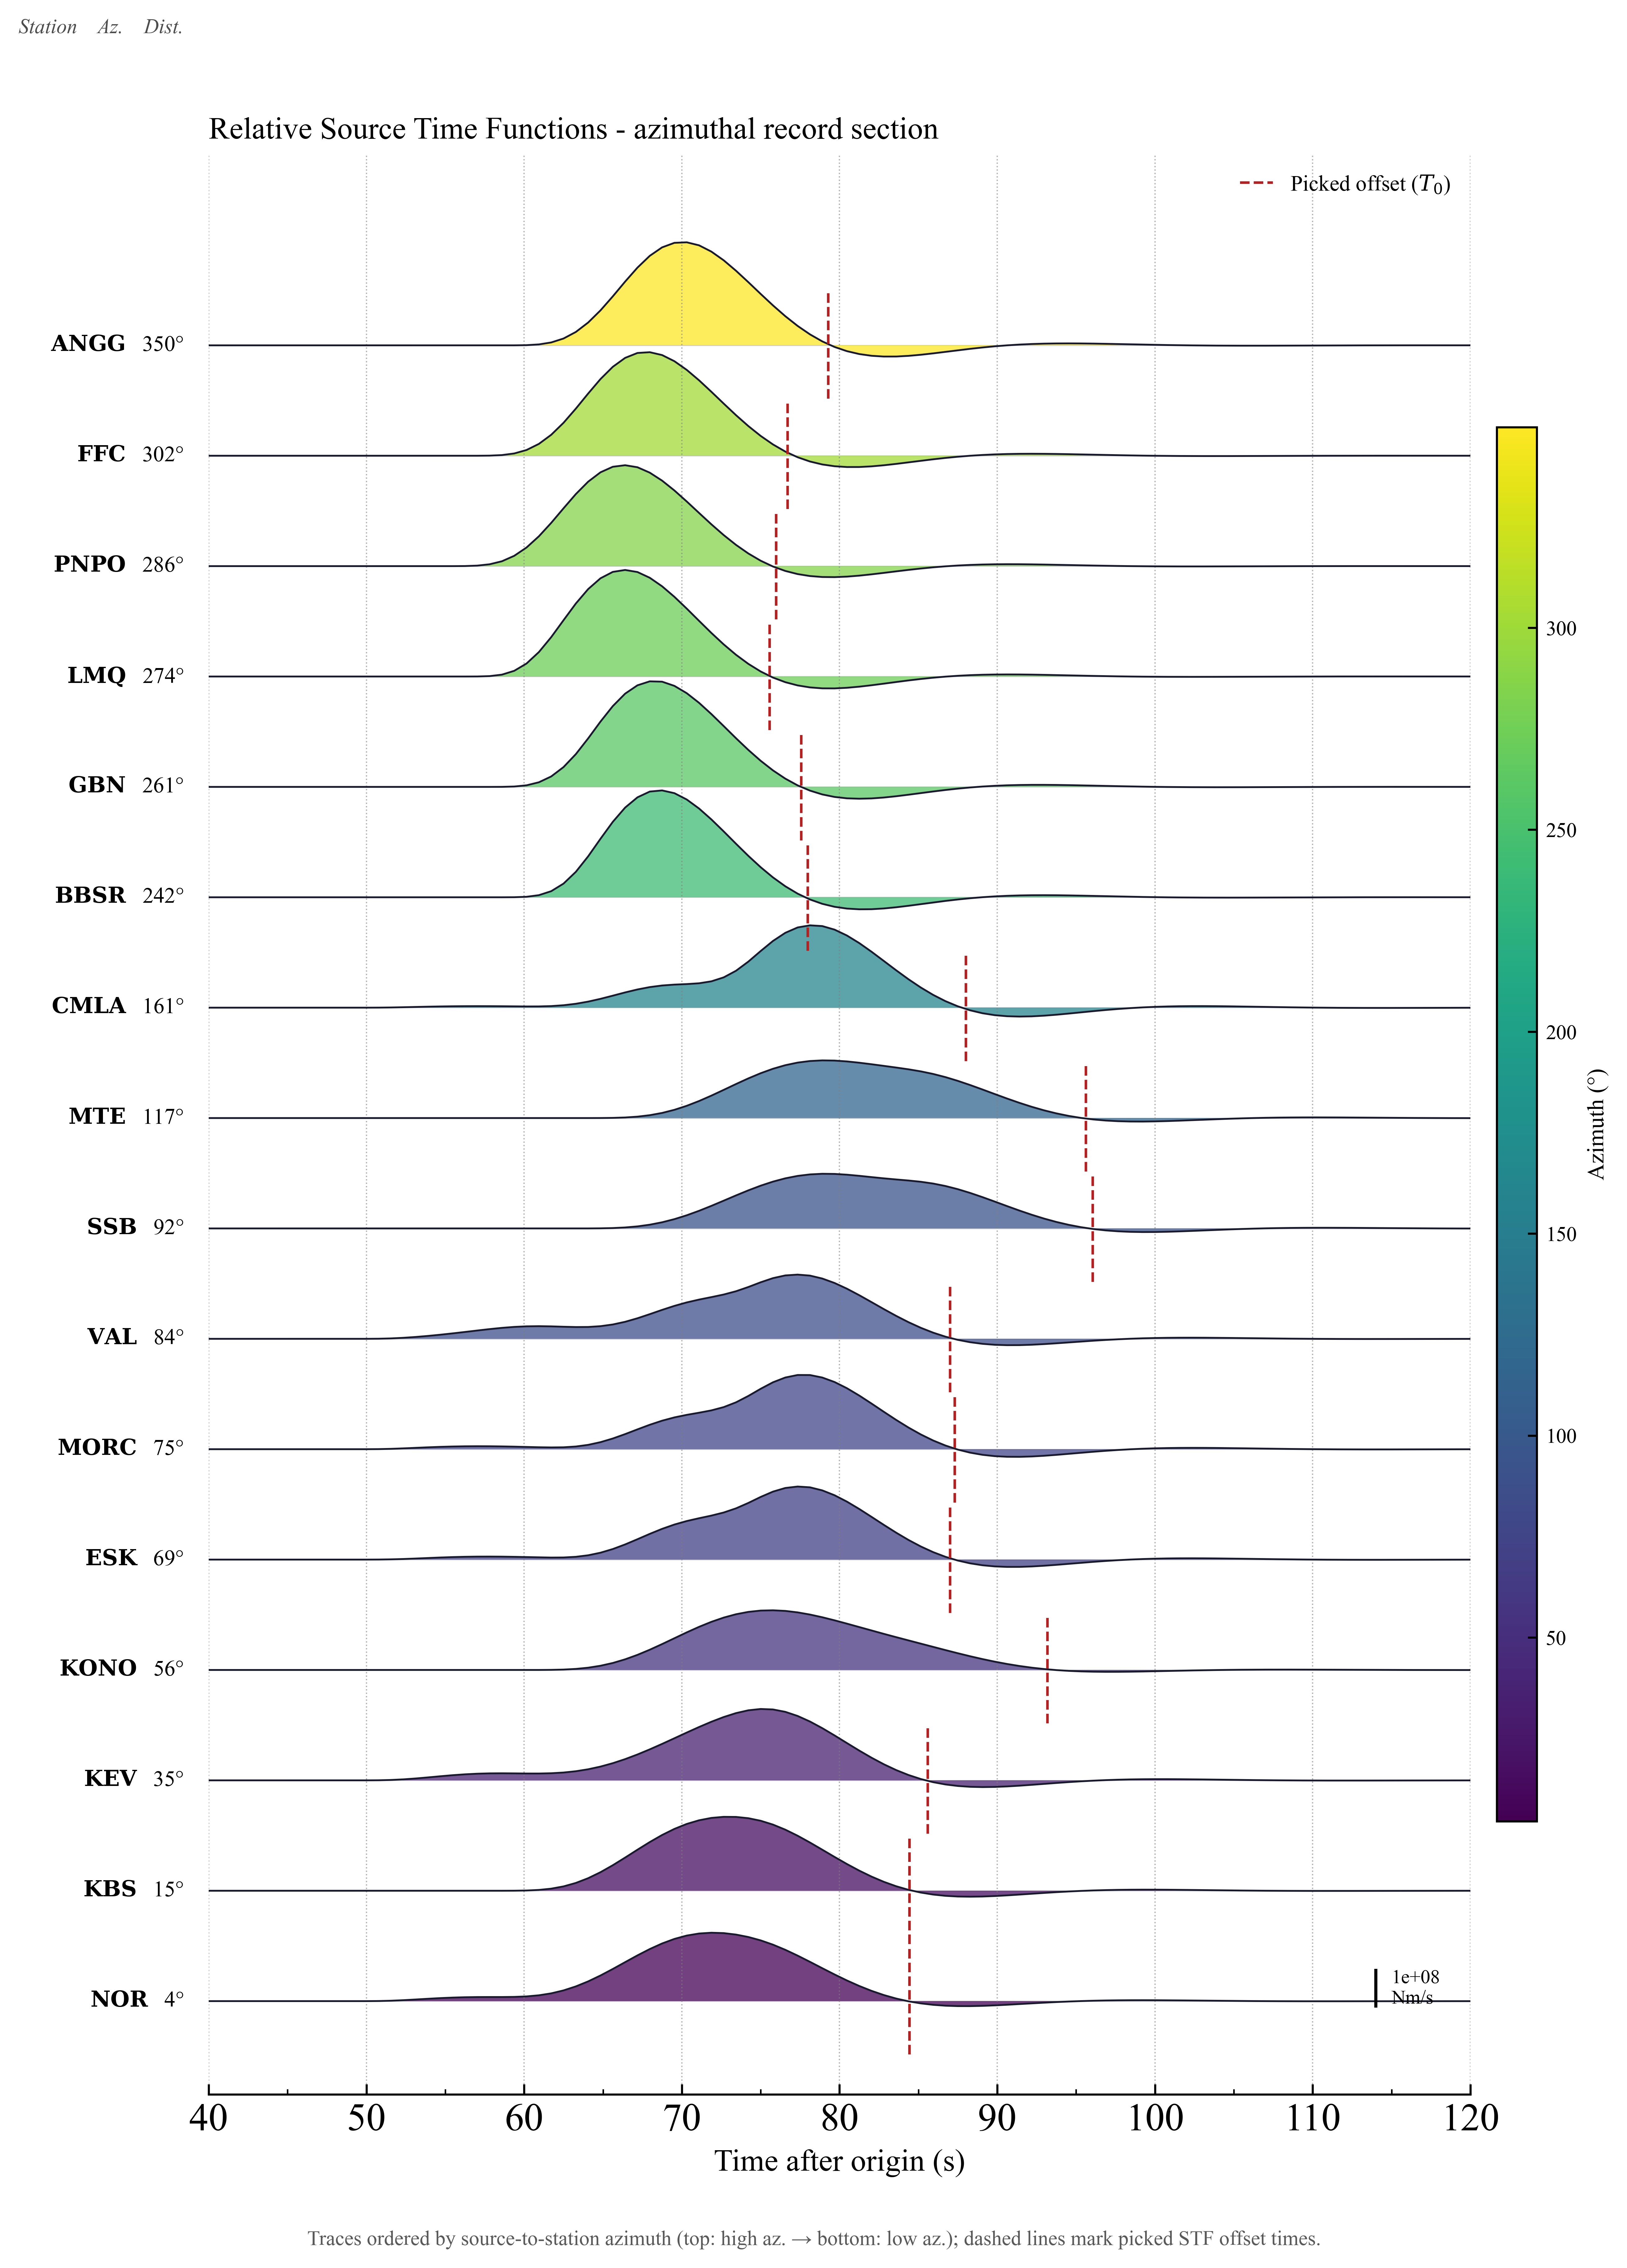
\includegraphics[width=\textwidth]{diagrams/2015_RSTF_azimuthal.png}
    %                 \caption{}
    %                 \label{fig:2015_rstf}
    %             \end{subfigure}
    %             \hfill
    %             \begin{subfigure}{0.5\textwidth}
    %                 % \centering
    %                 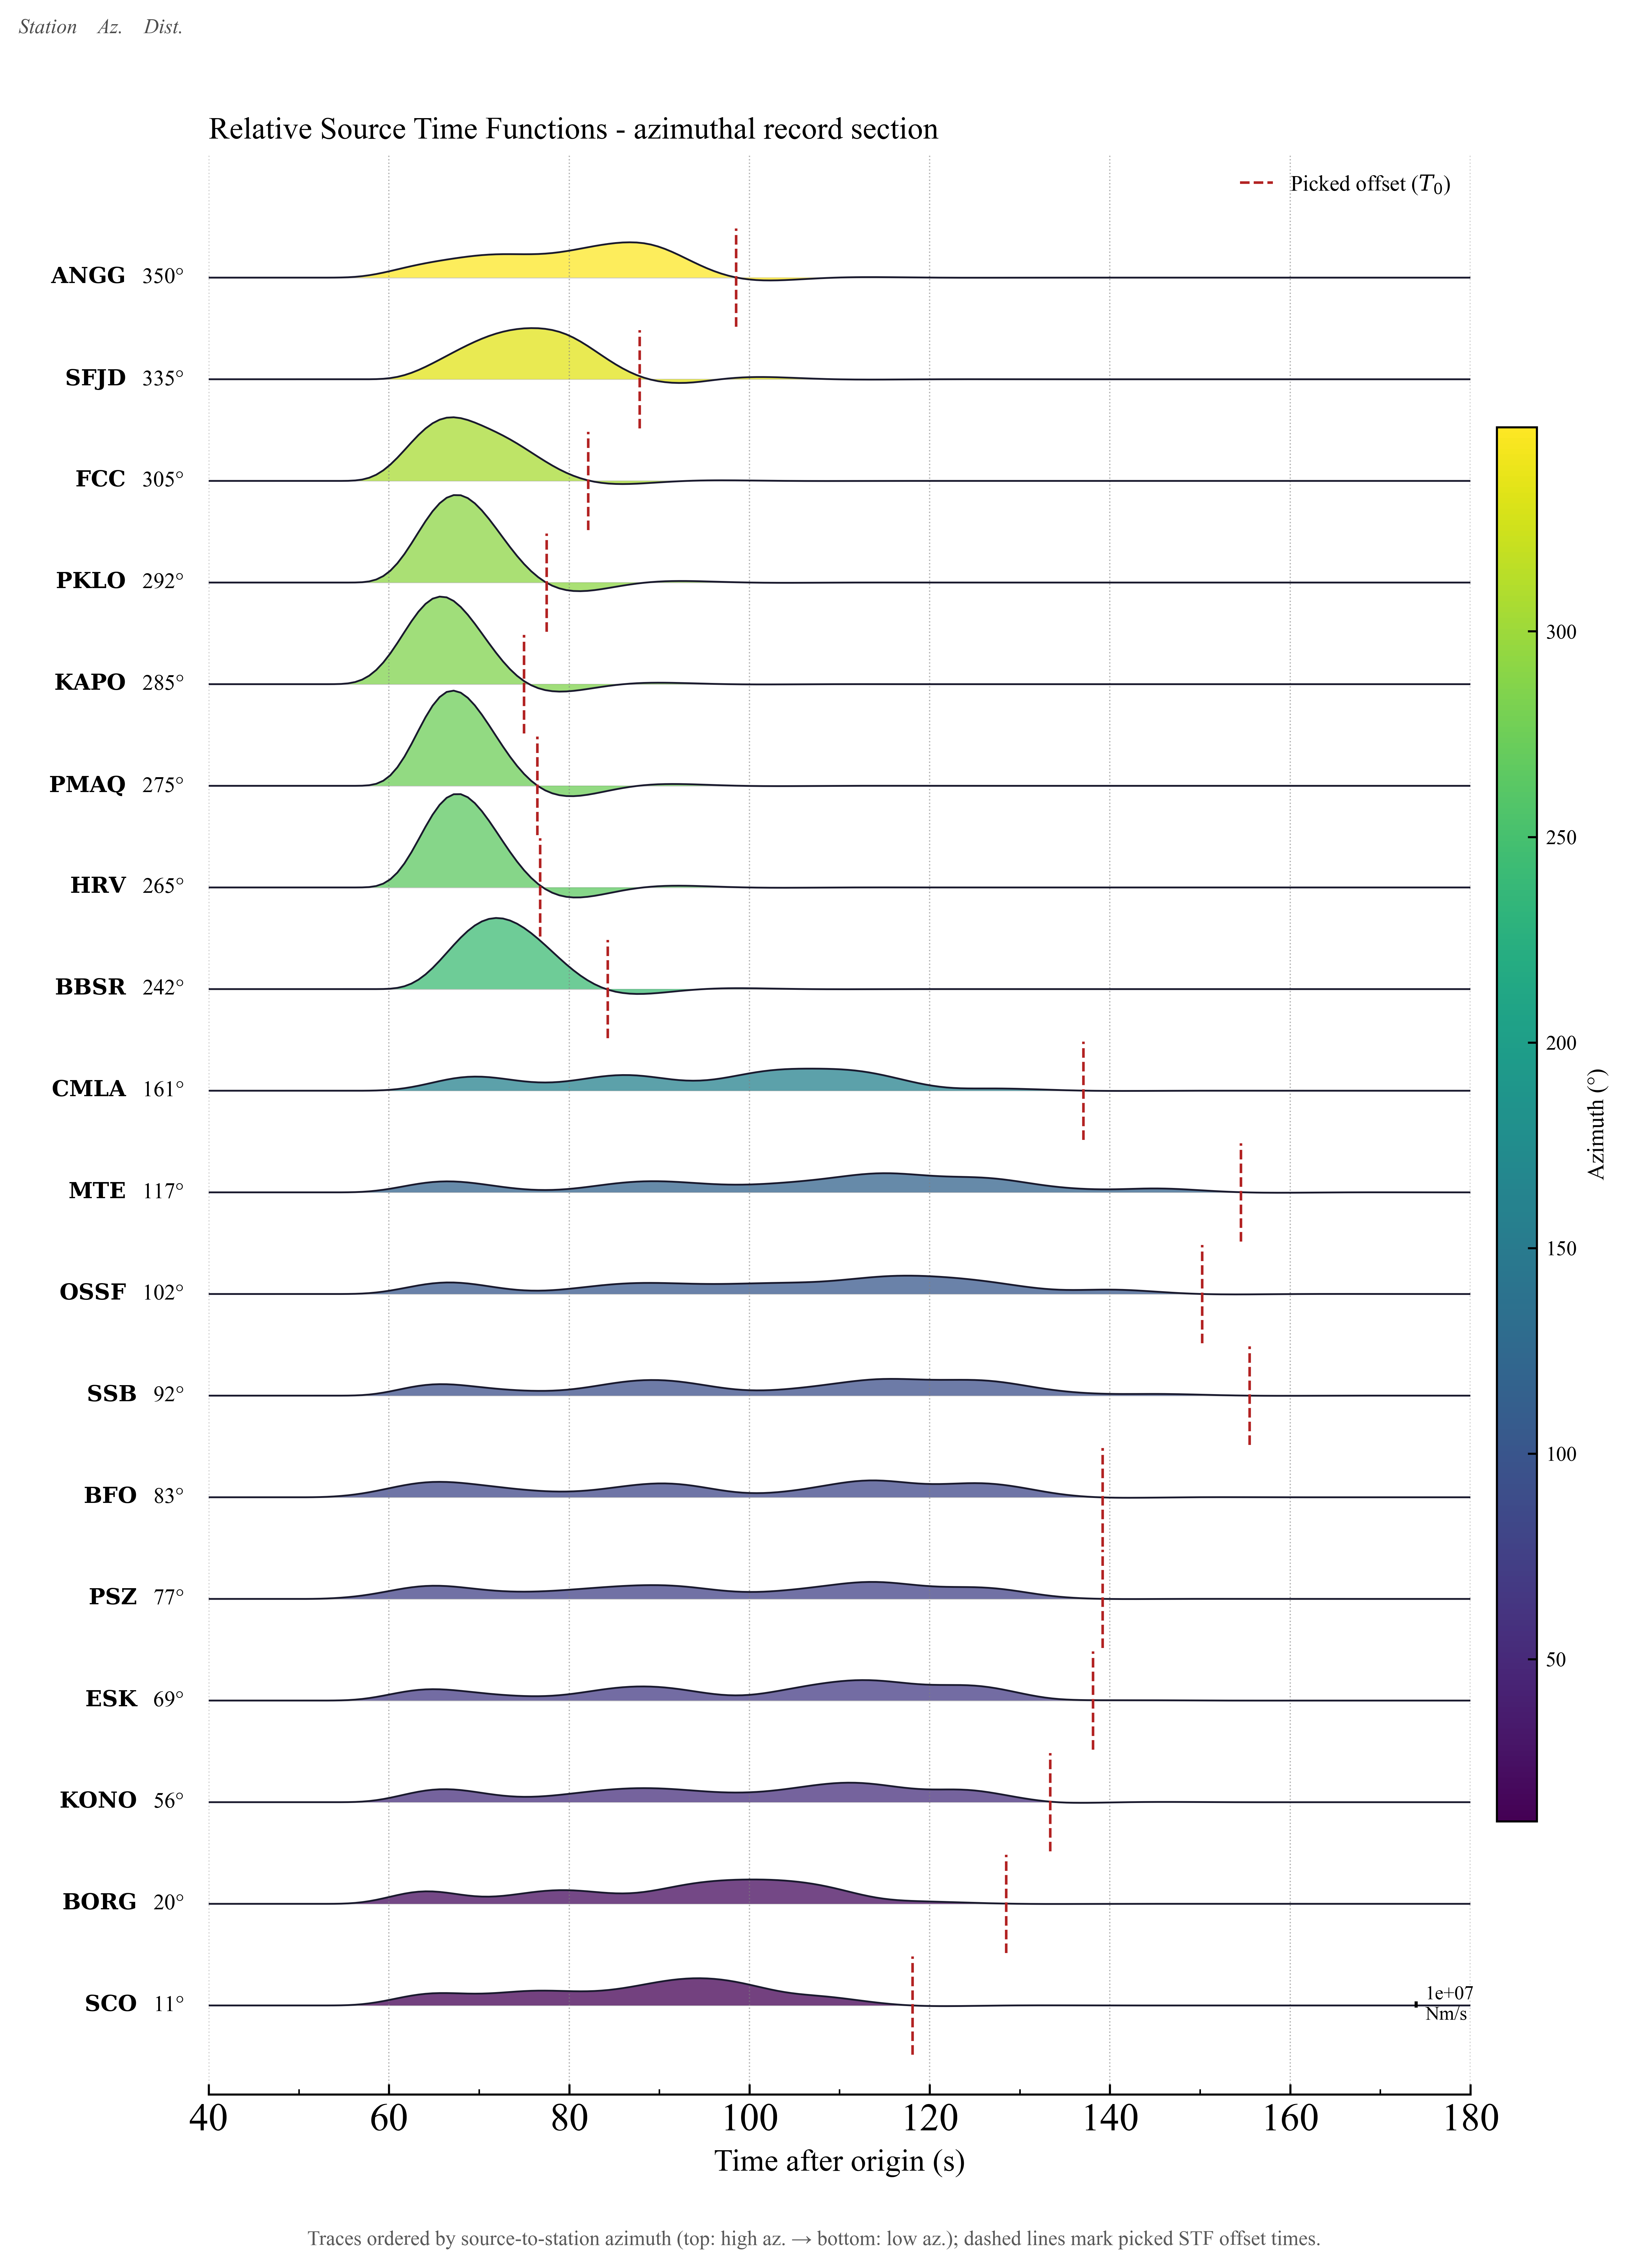
\includegraphics[width=\textwidth]{diagrams/2025_RSTF_azimuthal.png}
    %                 \caption{}
    %                 \label{fig:2025_rstf}
    %             \end{subfigure}
    %         \end{minipage}
        
    %     }
    %     \caption{Relative source time functions (RSTFs) from Love wave analysis (Projected Landweber Method). (a) RSTFs for the 2015 earthquake
    %      plotted as a function of station azimuth. The systematic variation in RSTF shape and duration with azimuth indicates a clear
    %      azimuthal dependence of the apparent source duration. (b) RSTFs for the 2025 earthquake are plotted using the same convention as in (a). Compared with 2015,
    %      the 2025 RSTFs exhibit more pronounced stretching and compression with azimuth, consistent with its longer source duration.}

    %     \label{fig:2015_2025_RSTF_comparison}

    % \end{figure}
\end{itemize}
\subsection{Methodology}
Will be written.
% \subsection{How the method is applied}
% \subsubsection{Data Selection and Teleseismic Preprocessing for Inversion}
% \begin{itemize}
%     \item 
%     \item For RSTF deconvolution, we retrieved data for a radius of 40 degrees around the epicentres of the 2015 and 2025 earthquakes.
%     \item For RSTF analysis, we selected the same earthquake which happened on 05/04/2025 as our EGF. Why this earthquake was selected
%      as EGF will be explained in the supporting information section.
%     \item Instrument response was also removed to maintain the homogeneity of the data.
%     \item For teleseismic phase picking, we selected data for a radius of 80 degrees to avoid upper-mantle triplications and core 
%     reflections \cite{heaton1990}.
%     \item The teleseismic P- and S-wave data were windowed for 70 and 115 s, respectively, with arrival-time uncertainties of 2.5 
%     and 7 s (for automated phase picking). The waveforms were processed using low- and broadband smoothing periods of 33 and 8 s, respectively, and 0.005Hz of 
%     third-order Butterworth low-pass filter is applied. Each filter was applied twice.
% \end{itemize}
\subsection{Finite-fault kinematic inversion}
\subsubsection*{Fault Plane Geometry}{}
% \begin{itemize}
%     \item \textbf{Fault plane geometry: } For both the inversion, we used same fault plane geomtry which is defined by: \\ \begin{itemize}
%         \item Strike: 098$^{\circ}$
%         \item Initial Dip: 80$^{\circ}$
%         \item Rake variation: $\pm 30^{\circ}$
%         \item Dip variation: $\pm 30^{\circ}$
%         \item 
%     \end{itemize}
% \end{itemize}

For both the 2015 and 2025 events, we adopted a consistent fault geometry and an $8 \times 8$~km subfault discretization, following the geometric 
constraints established by \cite{Aderhold2016}. Given their very similar focal depths, the hypocenters for both earthquakes were fixed at the same spatial
location—specifically at subfault 71. 
The defined fault plane spans $200$~km in length and $32$~km in width, with a strike of $98^\circ$, an initial dip of $75^\circ$, and an initial 
rake of $175^\circ$. To accommodate potential variations along the rupture surface during inversion, both rake and dip were permitted to deviate by 
up to $\pm 30^\circ$.

\subsubsection*{Inversion Configuration}
As initial configuration for the inversion, we set seismic moment of $5.6 \times 10^{26}~\mathrm{dyn\cdot cm}$ for the 2015 earthquake and
 $3 \times 10^{26}~\mathrm{Nm}$ for the 2025 earthquake, based on preliminary estimates from Mw 7.1. and Mw 6.9, respectively. The triangular source-time function
  for the subfaults is parameterized by 1 time window with a half-duration of 1.0 s, evaluated with a medium rigidity ($\mu$) of 4e11 dyn/cm², an initial
  synthetic triangle amplitude of 5e23 dyn·cm, a maximum allowable time delay of 30 s for 2015 and 60 s for 2025, a subfault point-source grid spacing
   ($\Delta x$) of 2 km, and a local 
  rupture propagation velocity of 3.5 km/s.Relative dataset weighting allocates 1.0 to teleseismic records and 1.0 to relative source-time functions (RSTFs),
   while assigning 0.0 to strong-motion, InSAR, GPS, and tsunami data as non-contributing. Inversion controls and regularization specify a moment minimization coefficient of 0.1,
    rupture velocity bounds from 2.0 km/s to 5.0 km/s, and spatial smoothing coefficients of 0.01 for slip, 0.0 
    for rupture velocity, 0.025 for rake variations, and 0.080 for dip variations. 
\paragraph*{}
This inversion solves for the spatial and temporal characteristics of
the rupture. The principal source parameters include: spatial distribution of slip amplitude, rake, spatial variation in fault dip, source time function (STF)
of the earthquake and rupture velocity.



\subsubsection{Comparison of the 2015 and 2025 earthquake slip distributions}
\begin{itemize}
    \item Slip distributions are plotted for both the 2015 and 2025 earthquakes. The slip distributions are compared to understand
     the similarities and differences in the rupture processes of the two events.
    \item Contours of the slips from both earthquakes are plotted in a single figure to visualize the spatial relationship between 
    the two slip distributions.
    \item To plot the contours we distributed the absolute slip values into 5 equal intervals starting from minumum slip of 8cm and 
    plotted the contours for both earthquakes in a single figure. 
\end{itemize}
\subsubsection{Comparison between source time functions of the 2015 and 2025 earthquakes}
\begin{itemize}
    \item The STFs are plotted for both earthquakes and the differences in the duration, peak amplitude, and overall shape of the STFs are analyzed. 
